\PassOptionsToPackage{usenames}{color}
\documentclass[11pt,letterpaper]{article}
\usepackage{etex} % remove ``No room for a new \dimen'' error

\usepackage{relsize} % relative font sizes (e.g. \smaller). must precede ACL style
\usepackage{style/naaclhlt2016}

%\naaclfinalcopy % Uncomment this line for the final submission
\def\naaclpaperid{***} %  Enter the naacl Paper ID here

% To expand the titlebox for more authors, uncomment
% below and set accordingly.
% \addtolength\titlebox{.5in}    

\usepackage[colorlinks=true,linkcolor=black,citecolor=black,filecolor=black,urlcolor=black]{hyperref}
\usepackage{natbib}
\newcommand{\citeposs}[1]{\citeauthor{#1}'s (\citeyear{#1})}

%\usepackage{times}
%\usepackage{latexsym}

\usepackage{framed}
\usepackage[boxed]{algorithm2e}
\renewcommand\AlCapFnt{\small}
\usepackage[small,bf,skip=5pt]{caption}
\usepackage{sidecap} % side captions
\usepackage{rotating}	% sideways

% Italicize subparagraph headings
\usepackage{titlesec}
\titleformat*{\subparagraph}{\itshape}
\titlespacing{\subparagraph}{%
  1em}{%              left margin
  0pt}{% space before (vertical)
  1em}%               space after (horizontal)

% Numbered Examples and lists
\usepackage{lingmacros}

\usepackage{enumitem} % customizable lists
\setitemize{noitemsep,topsep=0em,leftmargin=*}
\setenumerate{noitemsep,leftmargin=0em,itemindent=13pt,topsep=0em}
%%reduce space around captions
%\setlength{\abovecaptionskip}{1pt plus 1pt minus 1pt}
%\setlength{\belowcaptionskip}{1pt plus 1pt minus 1pt}

%\titlespacing*\section{0pt}{6pt plus 4pt minus 2pt}{4pt plus 2pt minus 2pt}
%\titlespacing*\subsection{1pt}{6pt plus 4pt minus 2pt}{0pt plus 2pt minus 2pt}
%\titlespacing*\subsubsection{1pt}{6pt plus 4pt minus 2pt}{0pt plus 2pt minus 2pt}
%\titlespacing*\paragraph{1pt}{6pt plus 4pt minus 2pt}{0pt plus 2pt minus 2pt}


\usepackage{textcomp}
% \usepackage{arabtex} % must go after xparse, if xparse is used!
%\usepackage{utf8}
% \setcode{utf8} % use UTF-8 Arabic
% \newcommand{\Ar}[1]{\RL{\novocalize #1}} % Arabic text

\usepackage{listings}

\lstset{
  basicstyle=\itshape,
  xleftmargin=3em,
  aboveskip=0pt,
  belowskip=-3pt, %-.5\baselineskip, % correct for extra paragraph break inserted after listing
  literate={->}{$\rightarrow$}{2}
           {α}{$\alpha$}{1}
           {δ}{$\delta$}{1}
           {(}{$($}{1}
           {)}{$)$}{1}
           {[}{$[$}{1}
           {]}{$]$}{1}
           {|}{$|$}{1}
           {+}{\ensuremath{^+}}{1}
           {*}{\ensuremath{^*}}{1}
}

\usepackage{amssymb}	%amsfonts,eucal,amsbsy,amsthm,amsopn
\usepackage{amsmath}

\usepackage{mathptmx}	% txfonts
\usepackage[scaled=.8]{beramono}
\usepackage[T1]{fontenc}
\usepackage[utf8x]{inputenc}

\usepackage{MnSymbol}	% must be after mathptmx

\usepackage{latexsym}

% Graphics
\usepackage{tikz}
\usetikzlibrary{arrows,positioning,calc} 



% Tables
\usepackage{array}
\usepackage{multirow}
\usepackage{booktabs} % pretty tables
\usepackage{multicol}
\usepackage{footnote}
\newcolumntype{H}{>{\setbox0=\hbox\bgroup}c<{\egroup}@{}} % hidden column

\usepackage{url}
\usepackage[usenames]{color}
\usepackage{xcolor}

% colored frame box
\newcommand{\cfbox}[2]{%
    \colorlet{currentcolor}{.}%
    {\color{#1}%
    \fbox{\color{currentcolor}#2}}%
}

\usepackage[normalem]{ulem} % \uline
\usepackage{colortbl}
\usepackage{graphicx}
\usepackage{subcaption}
%\usepackage{tikz-dependency}
%\usepackage{tikz}
%\usepackage{tree-dvips}
%\usetikzlibrary{arrows,positioning,calc} 
\usepackage{xytree}

\usepackage{xspace} % \xspace command for macros (inserts a space unless followed by punctuation)

\DeclareMathOperator*{\argmax}{arg\,max}
\DeclareMathOperator*{\argmin}{arg\,min}
\setlength\titlebox{4cm}    % Expanding the titlebox



% Author comments
\usepackage{color}
\newcommand\bmmax{0} % magic to avoid 'too many math alphabets' error
\usepackage{bm}
\definecolor{orange}{rgb}{1,0.5,0}
\definecolor{mdgreen}{rgb}{0,0.6,0}
\definecolor{mdblue}{rgb}{0,0,0.7}
\definecolor{dkblue}{rgb}{0,0,0.5}
\definecolor{dkgray}{rgb}{0.3,0.3,0.3}
\definecolor{slate}{rgb}{0.25,0.25,0.4}
\definecolor{gray}{rgb}{0.5,0.5,0.5}
\definecolor{ltgray}{rgb}{0.7,0.7,0.7}
\definecolor{purple}{rgb}{0.7,0,1.0}
\definecolor{lavender}{rgb}{0.65,0.55,1.0}

% Settings for algorithm listings
% \lstset{
%   language=Python,
%   upquote=true,
%   showstringspaces=false,
%   formfeed=\newpage,
%   tabsize=1,
%   commentstyle=\itshape\color{lavender},
%   basicstyle=\small\smaller\ttfamily,
%   morekeywords={lambda},
%   emph={upward,downward,tc},
%   emphstyle=\underbar,
%   aboveskip=0cm,
%   belowskip=-.5cm
% }
%\renewcommand{\lstlistingname}{Algorithm}


\newcommand{\ensuretext}[1]{#1}
\newcommand{\cjdmarker}{\ensuretext{\textcolor{green}{\ensuremath{^{\textsc{CJ}}_{\textsc{D}}}}}}
\newcommand{\nssmarker}{\ensuretext{\textcolor{magenta}{\ensuremath{^{\textsc{NS}}_{\textsc{S}}}}}}
\newcommand{\nasmarker}{\ensuretext{\textcolor{red}{\ensuremath{^{\textsc{NA}}_{\textsc{S}}}}}}
\newcommand{\dhmarker}{\ensuretext{\textcolor{red}{\ensuremath{^{\textsc{D}}_{\textsc{H}}}}}}
\newcommand{\ajmarker}{\ensuretext{\textcolor{purple}{\ensuremath{^{\textsc{A}}_{\textsc{J}}}}}}
\newcommand{\lkmarker}{\ensuretext{\textcolor{blue}{\ensuremath{^{\textsc{L}}_{\textsc{K}}}}}}
\newcommand{\swswmarker}{\ensuretext{\textcolor{orange}{\ensuremath{^{\textsc{S}}_{\textsc{S}}}}}}
\newcommand{\abmarker}{\ensuretext{\textcolor{purple}{\ensuremath{^{\textsc{A}}_{\textsc{B}}}}}}
\newcommand{\mcmarker}{\ensuretext{\textcolor{dkblue}{\ensuremath{^{\textsc{M}}_{\textsc{C}}}}}}
\newcommand{\arkcomment}[3]{\ensuretext{\textcolor{#3}{[#1 #2]}}}
%\newcommand{\arkcomment}[3]{}
\newcommand{\nss}[1]{\arkcomment{\nssmarker}{#1}{magenta}}
\newcommand{\aj}[1]{\arkcomment{\ajmarker}{#1}{purple}}
\newcommand{\dirk}[1]{\arkcomment{\dhmarker}{#1}{red}}
\newcommand{\lk}[1]{\arkcomment{\lkmarker}{#1}{blue}}
\newcommand{\swsw}[1]{\arkcomment{\swswmarker}{#1}{orange}}
\newcommand{\ab}[1]{\arkcomment{\abmarker}{#1}{purple}}
\newcommand{\mc}[1]{\arkcomment{\mcmarker}{#1}{dkblue}}
\newcommand{\wts}{\mathbf{w}}
\newcommand{\g}{\mathbf{g}}
\newcommand{\f}{\mathbf{f}}
\newcommand{\x}{\mathbf{x}}
\newcommand{\y}{\mathbf{y}}
\newcommand{\overbar}[1]{\mkern 1.5mu\overline{\mkern-1.5mu#1\mkern-1.5mu}\mkern 1.5mu} % \bar is too narrow in math
\newcommand{\cost}{c}

\usepackage{nameref}
\usepackage{cleveref}

% use \S for all references to all kinds of sections, and \P to paragraphs
% (sadly, we cannot use the simpler \crefname{} macro because it would insert a space after the symbol)
\crefformat{part}{\S#2#1#3}
\crefformat{chapter}{\S#2#1#3}
\crefformat{section}{\S#2#1#3}
\crefformat{subsection}{\S#2#1#3}
\crefformat{subsubsection}{\S#2#1#3}
\crefformat{paragraph}{\P#2#1#3}
\crefformat{subparagraph}{\P#2#1#3}
%\crefmultiformat{part}{\S#2#1#3}{ and~\S#2#1#3}{, \S#2#1#3}{, and~\S#2#1#3}
%\crefmultiformat{chapter}{\S#2#1#3}{ and~\S#2#1#3}{, \S#2#1#3}{, and~\S#2#1#3}
\crefmultiformat{section}{\S#2#1#3}{ and~\S#2#1#3}{, \S#2#1#3}{, and~\S#2#1#3}
\crefmultiformat{subsection}{\S#2#1#3}{ and~\S#2#1#3}{, \S#2#1#3}{, and~\S#2#1#3}
\crefmultiformat{subsubsection}{\S#2#1#3}{ and~\S#2#1#3}{, \S#2#1#3}{, and~\S#2#1#3}
\crefmultiformat{paragraph}{\P\P#2#1#3}{ and~#2#1#3}{, #2#1#3}{, and~#2#1#3}
\crefmultiformat{subparagraph}{\P\P#2#1#3}{ and~#2#1#3}{, #2#1#3}{, and~#2#1#3}
%\crefrangeformat{part}{\mbox{\S\S#3#1#4--#5#2#6}}
%\crefrangeformat{chapter}{\mbox{\S\S#3#1#4--#5#2#6}}
\crefrangeformat{section}{\mbox{\S\S#3#1#4--#5#2#6}}
\crefrangeformat{subsection}{\mbox{\S\S#3#1#4--#5#2#6}}
\crefrangeformat{subsubsection}{\mbox{\S\S#3#1#4--#5#2#6}}
\crefrangeformat{paragraph}{\mbox{\P\P#3#1#4--#5#2#6}}
\crefrangeformat{subparagraph}{\mbox{\P\P#3#1#4--#5#2#6}}
% for \label[appsec]{...}
\crefname{part}{Part}{Parts}
\Crefname{part}{Part}{Parts}
\crefname{chapter}{ch.}{ch.}
\Crefname{chapter}{Ch.}{Ch.}
\crefname{figure}{figure}{figures}
\crefname{appsec}{appendix}{appendices}
\Crefname{appsec}{Appendix}{Appendices}
\crefname{algocf}{algorithm}{algorithms}
\Crefname{algocf}{Algorithm}{Algorithms}
\crefname{enums,enumsi}{example}{examples}
\Crefname{enums,enumsi}{Example}{Examples}
\crefname{}{example}{examples} % lingmacros \toplabel has no internal name for the kind of label
\Crefname{}{Example}{Examples}
\crefformat{enums}{(#2#1#3)}
\crefformat{enumsi}{(#2#1#3)}
\crefformat{}{(#2#1#3)}
\crefrangeformat{enums}{\mbox{(#3#1#4--#5#2#6)}}
\crefrangeformat{enumsi}{\mbox{(#3#1#4--#5#2#6)}}

\ifx\creflastconjunction\undefined%
\newcommand{\creflastconjunction}{, and\nobreakspace} % Oxford comma for lists
\else%
\renewcommand{\creflastconjunction}{, and\nobreakspace} % Oxford comma for lists
\fi%

\newcommand*{\Fullref}[1]{\hyperref[{#1}]{\Cref*{#1}: \nameref*{#1}}}
\newcommand*{\fullref}[1]{\hyperref[{#1}]{\cref*{#1}: \nameref{#1}}}
\newcommand{\fnref}[1]{footnote~\ref{#1}} % don't use \cref{} due to bug in (now out-of-date) cleveref package w.r.t. footnotes
\newcommand{\Fnref}[1]{Footnote~\ref{#1}}


% Space savers
% From http://www.eng.cam.ac.uk/help/tpl/textprocessing/squeeze.html
% \addtolength{\dbltextfloatsep}{-.5cm} % space between last top float or first bottom float and the text.
% \addtolength{\intextsep}{-.5cm} % space left on top and bottom of an in-text float.
% \addtolength{\abovedisplayskip}{-.5cm} % space before maths
% \addtolength{\belowdisplayskip}{-.5cm} % space after maths
% %\addtolength{\topsep}{-.5cm} %space between first item and preceding paragraph
%\setlength{\belowcaptionskip}{-.5cm}


% customize \paragraph spacing
% \makeatletter
% \renewcommand{\paragraph}{%
%   \@startsection{paragraph}{4}%
%   {\z@}{.2ex \@plus 1ex \@minus .2ex}{-1em}%
%   {\normalfont\normalsize\bfseries}%
% }
% \makeatother


% Special macros
\newcommand{\tg}[1]{\texttt{#1}}	% tag name
\newcommand{\sst}[1]{\textsc{#1}} % supersense category
\newcommand{\gfl}[1]{%\renewcommand\texttildelow{{\lower.74ex\hbox{\texttt{\char`\~}}}} % http://latex.knobs-dials.com/
\mbox{\textsmaller{\texttt{#1}}}}	% supersense tag symbol
%\newcommand{\lex}[1]{\textsmaller{\textsf{\textcolor{slate}{\textbf{#1}}}}}	% example lexical item 
\newcommand{\tagdef}[1]{#1\hfill} % tag definition
\newcommand{\tagt}[2]{\ensuremath{\underset{\textrm{\textlarger{\tg{#2}}}\strut}{\w{#1}\rule[-.3\baselineskip]{0pt}{0pt}}}} % tag text (a word or phrase) with an SST. (second arg is the tag)
\newcommand{\tagtt}[3]{\begin{tabular}{@{\hspace{2pt}}c@{\hspace{2pt}}} \texttt{#2}\\ #1 \\ \texttt{#3}\end{tabular}}
\newcommand{\tagts}[3]{\begin{tabular}{@{\hspace{2pt}}c@{\hspace{2pt}}} \texttt{#2\vphantom{\textlarger{Ĩ}}}\\ #1 \\ \sst{#3}\end{tabular}}
\newcommand{\tagtss}[5]{\begin{tabular}{@{\hspace{2pt}}c@{\hspace{2pt}}} \texttt{#2\vphantom{\textlarger{Ĩ}}}\\ \sst{#3}\vphantom{X} \\ \textbf{#1}\vphantom{lp} \\ \sst{#5}\vphantom{X} \\ \texttt{#4\vphantom{\textlarger{Ĩ}}}\end{tabular}}
\newcommand{\tgt}[2]{\ensuremath{\underset{\text{\textlarger{#2}\strut}}{\text{#1\rule[-.3\baselineskip]{0pt}{\baselineskip}}}}} % tag text (a word or phrase, not underlined) with a label. (second arg is the label)
\newcommand{\glosst}[2]{\ensuremath{\underset{\textrm{#2}}{\textrm{#1}}}} % gloss text (a word or phrase) (second arg is the gloss)
\newcommand{\AnnA}[0]{\mbox{\textbf{Ann-A}}} % annotator A
\newcommand{\AnnB}[0]{\mbox{\textbf{Ann-B}}} % annotator B
\newcommand{\sys}[1]{\mbox{\textbf{#1}}}   % name of a system (one of our experimental conditions)
\newcommand{\dataset}[1]{\mbox{\textsc{#1}}}	% one of the datasets in our experiments
\newcommand{\datasplit}[1]{\mbox{\textbf{#1}}}	% portion one of the datasets in our experiments

\newcommand{\w}[1]{\textit{#1}}	% word
\newcommand{\lex}[1]{\textit{#1}} % lexical item
\newcommand{\tweet}[1]{\textsf{#1}}	% tweet
\newcommand{\twbank}[0]{\textsc{Tweebank}\xspace}
\newcommand{\foster}[0]{\textsc{Foster}\xspace}
\newcommand{\twparser}[0]{\textsc{Tweeboparser}\xspace}
\newcommand{\tat}[0]{\textasciitilde}
\newcommand{\backtick}[0]{\textasciigrave}

%\newcommand{\finalversion}[1]{#1}
\newcommand{\finalversion}[1]{}
\newcommand{\shortversion}[1]{}
\newcommand{\considercutting}[1]{#1}
\newcommand{\longversion}[1]{#1} % ...if only there were more space...

\hyphenation{WordNet}
\hyphenation{WordNets}
\hyphenation{VerbNet}
\hyphenation{FrameNet}
\hyphenation{SemCor}
\hyphenation{SemEval}
\hyphenation{PennConverter}
\hyphenation{TurboParser}
\hyphenation{Tweebo-parser}
\hyphenation{Twee-bank}
\hyphenation{an-aly-sis}
\hyphenation{an-aly-ses}
\hyphenation{news-text}
\hyphenation{base-line}
\hyphenation{de-ve-lop-ed}
\hyphenation{comb-over}


\title{SemEval-2016 Task~10:\\ Detecting Minimal Semantic Units and their Meanings (DiMSUM)}

\author{
Nathan Schneider \\
		School of Informatics\\
	   	University of Edinburgh\\
	    Edinburgh, UK\\
	    {\tt nschneid@inf.ed.ac.uk} \And
Dirk Hovy \quad Anders Johannsen\\
Center for Language Technology\\
University of Cophenhagen\\
Copenhagen, Denmark\\
{\tt \{krx628,ajohannsen\}@hum.ku.dk} \And
Marine Carpuat\\
Computer Science Dept.\\
University of Maryland\\
College Park, Maryland, USA\\
{\tt marine@cs.umd.edu}}


\date{}

\begin{document}
% \nss{Note: this document uses natbib rather than the standard ACL bib macros: 
% According to \citet{baldwin-10}, statistical association measures 
% are one technique for extracting MWE types \citep[cf.][\emph{inter alia}]{pecina-10}.}
\naaclfinalcopy % show authors
\maketitle
\global\naaclfinalfalse % turn on header/line numbers for review

\begin{abstract}
This task adopts an explicit yet broad-coverage paradigm for lexical semantics, representing
multiword expressions and supersenses (coarse-grained classes) in an integrated fashion.
Nine systems were submitted; the best scored .57 $F_1$ in a multi-domain evaluation setting, 
indicating that the task remains largely unresolved. 
An error analysis reveals that a large number of instances in the data set are either hard cases 
which no systems get right or easy cases that all systems correctly solve.
%We propose a SemEval~2016 Shared Task 
%of analyzing the lexical semantics of English sentences 
%in a broad-coverage fashion. 
%The task formulation consists of two closely related steps which can be performed jointly:
%(a)~chunking tokens within sentences into \textbf{multiword expressions}, and 
%(b)~assigning coarse \textbf{supersense} labels to all noun and verb expressions. 
%The evaluation will build upon recently annotated datasets in two social web genres.
%\longversion{We expect that the task formulation will foster engagement across 
%multiple subcommunities of computational semantics, 
%and facilitate empirical comparison of methodologically diverse systems.}
\end{abstract}

\section{Introduction}\label{sec:intro}


% Broad-coverage NLP techniques such as XXX\dirk{Nathan, could you make clear what broad coverage is?} have
% become mainstream for several aspects of language---including morphology, syntax, 
% and some areas of semantics (notably, named entity recognition, %\nss{2002/2003}
% semantic role labeling, %\nss{2004/2005/2008/2009} 
% and coreference resolution). %\nss{2011/2012}
% %, thanks in part to previous SemEval shared tasks,

Bread-and-butter grammatical analysis tasks in contemporary NLP---part-of-speech tagging, for example---are \emph{comprehensive}, 
operating under the assumption that all grammatically-relevant parts of a sentence  
will be substantively analyzed. (We do not expect POS taggers to only know about a subset of the parts of speech in the language.) 
Furthermore, for manual annotation, 
POS tags accommodate unseen words, and most adapt readily to new text genres.
These factors, taken together, indicate a representation achieves \emph{broad coverage}. 

Explicit analysis of lexical semantics, by contrast, has been more difficult to scale 
to broad coverage.
The dominant paradigm of fine-grained word sense disambiguation, WordNet \citep{wordnet}, 
is difficult to annotate in corpora, results in considerable data sparseness, 
and does not readily generalize to out-of-vocabulary words.
While the main corpus with WordNet senses, 
SemCor \citep{semcor}, does reflect several text genres, it is hard
to expand its annotations to new genres, such as social web text 
or transcribed speech.
This severely limits the applicability of SemCor-based NLP tools 
and restricts opportunities for linguistic studies of lexical semantics in corpora.

\finalversion{\nss{do we want to say something about insights from MT? this needs work:}
Consequently,  \citet{carpuat-05,resnik-06} found that traditional, fine-grained word sense disambiguation 
did indeed \emph{not} improve machine translation. 
\nss{TODO}However, abstracting the senses and moving to multi-word does \citep{chan-07,carpuat-07,lefever-10}.
}

%The goal of this task is therefore to establish a broad-coverage paradigm for lexical semantic analysis that works on a variety of genres.
%translations in a second language replaced abstract word senses, 
%and the single-word disambiguation targets were replaced by the multiword phrases used 
%by translation systems 

We report on the DiMSUM~2016 shared task,\footnote{\url{http://dimsum16.github.io/}} which challenged participants to analyze the lexical semantics 
of English sentences with a tagset integrating
\textbf{multiword expressions} and \textbf{noun and verb supersenses} \citep[following][]{schneider-15}, 
on multiple nontraditional genres of text. 
By moving away from fine-grained sense inventories and lexicalized, language-specific\footnote{Though our dataset is limited to English, the representation is applicable to other languages: see \cref{sec:integration}.} annotation,
we take a step in the direction of broad-coverage, coarse-grained lexical semantic analysis. 
We believe this departure from the classical lexical semantics paradigm 
will ultimately prove fruitful for a variety of NLP applications in a variety of genres. 
%to establish a broad-coverage paradigm for lexical semantic analysis that works on a variety of genres.

% \nss{motivation: lexical semantic analysis of MWEs and supersenses in English. 
% semantics is a hot topic.
% highlights: (a) broad-coverage---not too far from NER; hopefully avoid some of the limitations of traditional WSD. 
% (b) robust to domain---in fact, evaluation consists of 2 social web domains.
% (c) potential to benefit from many different NLP techniques, including sequence tagging/chunking, 
% parsing, distributional word representations, language models, 
% use of language resources such as WordNet, (other buzzwords?)}

%\paragraph{Summary}
%To date, many of the analysis problems in computational lexical semantics are limited in scope, due to granularity and coverage.
%We integrate broad-coverage MWE identification with supersense tagging 
The integrated lexical semantic representation (\cref{sec:integration}, \cref{sec:rep})
has been annotated in an extensive benchmark dataset comprising several nontraditional domains (\cref{sec:data}).
Objective, controlled evaluation procedures (\cref{sec:eval})
facilitate a comparison of the 9~systems submitted as part of the official task (\cref{sec:results}).
While the systems range in performance, all are below 60\% in our composite evaluation, 
suggesting that further work is needed to make progress on this difficult task.



% \nss{encourage creativity of solutions}
% Semantic analysis is a powerful and promising topic, but it has been largely confined to news text, 
% i.e., standardized text written mostly in English. 
% By including a relatively new and heterogeneous domain like Twitter in the data, 
% we want to encourage creative approaches that go beyond the tried and true newswire-trained approach, 
% and open the community to wider applications. 

% This task would capitalize on current enthusiasm for semantics in NLP, 
% providing a testbed for a wide variety of technical approaches---these could include 
% linguistic feature engineering; comparing sequence models to hierarchical parsing models, or their combination 
% with joint decoding \citep{le_roux-14}; domain adaptation \citep{johannsen-14}; 
% type supervision; word clustering\slash representation learning \citep{grave-13}; 
% collocation extraction \citep{pecina-10,ramisch-12}; 
% language modeling; or other methods that exploit additional resources.

% This is a new task. 
% We believe it will attract strong participation from researchers in lexical semantics, 
% structured prediction, (semi)supervised learning, domain adaptation, and social media NLP. 
% To gauge interest, we reached out informally to a number of leaders in the field, 
% asking for feedback on the idea. Several of them have indicated that they consider this 
% a worthwhile task and will consider participating if it is accepted.
% As a rough estimate, we think it would attract participation from about 20~teams.
% If it is accepted, we will publicize the task widely in order to recruit as much participation as possible.


\section{Background}\label{sec:integration}
\textbf{Multiword expressions.} 
Most contemporary approaches to syntactic and semantic analysis
treat space-separated words as the basic units of structure. 
%It has even been suggested that dependency syntax, for example, 
%offers a good approximation of semantic structure.
However, this fails to reflect 
the basic units of meaning for sentences with non-compositional or idiosyncratic expressions, such as:
%\begin{enumerate}[leftmargin=*,labelsep=2em,label=(\arabic*),before=\raggedright]
\begin{itemize}[labelindent=2em]
\item[(1)] The staff {\color{red}leaves} {\color{blue}a lot} {\color{red}to be desired} .
\item[(2)] \raggedright I googled restaurants in the area and {\color{red}Fuji Sushi} {\color{blue}came up} and reviews were great so I {\color{mdgreen}made a} {\color{orange}carry out} {\color{mdgreen}order} of : L 17 .
\end{itemize}
In these sentences, \lex{a lot}, \lex{leaves\ldots to be desired}, 
\lex{Fuji Sushi}, \lex{came up}, \lex{made\ldots order}, and \lex{carry out}
are all \textbf{multiword expressions} (MWEs): their combined meanings can be thought of as ``prepackaged'' 
in a single lexical expression that happens to be written with spaces.
%\footnote{This is not to say that MWEs cannot have ``normal'' 
%syntactic structure; some are more fixed in their form while others are quite flexible. 
%For instance, \lex{make\ldots order} can be passivized just like canonical transitive verb phrases.}
MWEs such as these have attracted a great deal of attention 
within computational semantics; see \citet{baldwin-10} for a review.
\Citet{schneider-14-corpus} introduced an English corpus resource annotated for heterogenous MWEs, 
suitable for training and evaluating general-purpose MWE identification systems \citep{schneider-14}.
Prior to that, most MWE evaluations were focused on particular constructions such as noun compounds \citep[recently:][]{constant-11,green-12,ramisch-12,vincze-13},
though the corpus and identification system of \citet{vincze-11} targets several kinds of MWEs.

Importantly, the MWEs in \citeposs{schneider-14-corpus} corpus are not required to be contiguous, 
but may contain \textbf{gaps} (viz.: \lex{made\ldots order}). The corpus also contains qualitative labels indicating the strength of MWEs, either \textbf{strong} (mostly non-compositional) or \textbf{weak} (compositional but idiomatic). For simplicity we only include strong MWEs in this task.

\textbf{Supersenses.}
% \longversion{
% Ideally, a lexical semantic representation would apply to a large number of word types 
% while being sufficiently fine-grained to disambiguate words with multiple meanings. 
% %A representation represents good coverage if it provides labels for most word classes. 
% %It offers sufficient distinction if it allows one to group words into clusters, 
% %in order to make generalizations about semantic classes. 
% A good meaning representation should also group together related meanings from different words. 
% %is typically anti-correlated with the number of available labels.
% These ideals are sometimes at odds:  \nss{\ldots}
% 
% Popular representations are named-entity tags and WordNet \citep{wordnet} word senses. 
% However, both present a problem in one of the desired aspects. 
% Named entity tags have a reasonable distinction, and are thus frequently used to find entities of a certain type. 
% However, as the name already suggests, this representation is limited to (proper) nouns, and even though high-coverage gazetteers can be found for named entity recognition, the task has thus inherently poor coverage. 
% Word senses, on the other hand, cover all content word classes. 
% However, they are lemma-specific (i.e., sense number two of \emph{house} and \emph{building} are not the same), 
% and do not allow for generalization to larger groups.\nss{not true of WordNet, because the hierarchy allows generalization. 
% I think the problems with the WordNet-style approach are (a)~it is hard to agree on/annotate with fine-grained senses, 
% and (b)~it is hard to extend the lexicon to cover OOV words that might occur in new domains (let alone other languages).}
% }
As noted above, relying on WordNet-like fine-grained, lexicalized senses 
creates problems for scalability and extensibility to new domains and languages. 
Named entity recognition (NER) does not suffer from these problems, but its classes---a small number of coarse-grained classes---only apply to named entities, not verbs, adjectives, or common nouns.
They therefore provide far from complete coverage in a corpus.

Noun and verb \textbf{supersenses}
offer a middle ground in granularity: they generalize 
named entity classes to cover all nouns (with 26~classes), but also cover verbs (15~classes)---see \cref{tbl:supersenses}---and provide a human-interpretable high-level clustering. WordNet supersenses for adjectives and adverbs nominally exist, 
but are based on morphosyntactic rather than semantic properties.  
There is, however, recent work on developing supersense taxonomies for English adjectives and prepositions \citep{tsvetkov-14,schneider-15-law}.

The inventory for nouns and verbs originates from the top-level organization of WordNet,
but can be applied directly to annotate new data---including out-of-vocabulary words 
in English or other languages \citep{schneider-12,johannsen-14}. 
Similar to NER, supersense tagging approaches have generally used statistical sequence models 
and have been evaluated in English, Italian, Chinese, Arabic, and Danish.\footnote{Evaluations used 
English SemCor \citep{ciaramita-06,paas-09}, 
English-Italian MultiSemCor \citep{picca-08,picca-09,attardi-10}, 
the Italian Syntactic-Semantic Treebank and Italian Wikipedia \citep{attardi-10,rossi-13}, 
Chinese Cilin \citep{qiu-11},  
Arabic Wikipedia \citep{schneider-13}, and the Danish CLARIN Reference Corpus \citep{martinez-15}.}

Features based on supersenses have also been exploited in downstream semantics tasks\longversion{ 
such as preposition sense disambiguation, noun compound interpretation, and metaphor detection} 
\citep{ye-07,hovy2010,tratz-10,hovy-2013identifying,tsvetkov-13}. 

\begin{table}\centering\small
\resizebox{ \columnwidth }{!}{
\begin{tabular}{>{\sst\bgroup}l<{\egroup}>{\sst\bgroup}l<{\egroup}>{\sst\bgroup}l<{\egroup}}
n:Tops	&	n:object	&	v:cognition\\
n:act	&	n:person	&	v:communication\\
n:animal	&	n:phenomenon	&	v:competition\\
n:artifact	&	n:plant	&	v:consumption\\
n:attribute	&	n:possession	&	v:contact\\
n:body	&	n:process	&	v:creation\\
n:cognition	&	n:quantity	&	v:emotion\\
n:communication	&	n:relation	&	v:motion\\
n:event	&	n:shape	&	v:perception\\
n:feeling	&	n:state	&	v:possession\\
n:food	&	n:substance	&	v:social\\
n:group	&	n:time	&	v:stative\\
\cline{2-2}
n:location	&	v:body	&	v:weather\\
n:motive	&	v:change	&	
\end{tabular}
}% resize
\caption{The 41 noun and verb supersenses in WordNet.}
\label{tbl:supersenses}
\end{table}

% \longversion{
% The \textbf{supersense} categories for nouns and verbs, \cref{tbl:supersenses},
% are also derived from WordNet, but represent a higher level in the taxonomy. 
% They originated from a higher-level clustering of nouns and verbs into groups, 
% and thus have good coverage.\footnote{Supersenses for adjectives and adverbs nominally exist, 
% but are based on morphosyntactic rather than semantic properties. 
% There is, however, recent work on developing a taxonomy for English adjective supersenses \citep{tsvetkov-14}.}
% Since they group individual word senses into larger groups, they allow for distinction beyond the lemma level, 
% i.e., they assign the same supersense to words with different word senses. Supersenses thus provide 
% human-interpretable high-level clustering information, and have mostly been used as features in other tasks, 
% such as preposition sense disambiguation, noun compound interpretation, and metaphor detection 
% \cite{Ye:Baldwin:2007,Tratz:Hovy:2010,Tsvetkov:ea:2013}. 
% 
% The task of supersense tagging was first introduced by \citep{Ciaramita:Altun:2006EMNLP}, 
% who used 5-fold cross validation on {\sc SemCor} to evaluate their model (structured 1st order discriminative). 
% Their evaluation also included a held-out development set on each fold that was used to estimate the number of epochs 
% and additional training data containing only verbs. Their overall $F_1$ score on {\sc SemCor} was 77.1.
% Reichartz and Paa\ss{} \citep{Reichartz:Paass:2008ECMLPKDD,Paass:Reichartz:2009SIAM} 
% reached an $F_1$ score of 80.2, using CRFs and additional features.
% 
% There has been relatively little recent work on supersense tagging, and to the best of our knowledge, all of it has been mostly limited to standard English\footnote{With few exceptions such as \cite{schneider-12,schneider-13}.} ({\sc SemCor} and {\sc SensEval}). We are not aware of any previous work on word sense disambiguation for Twitter. Our hope is that this task makes the problem more attractive to a wider audience to reach more languages and domains.
% }


\textbf{Relationship between MWEs and supersenses.}
We believe that MWEs and supersenses should be tightly coupled:
idiomatic combinations such as MWEs are best labeled holistically,
since their joint supersense category will often differ from that of the individual words.
For example, \lex{spill the beans} in its literal interpretation
would receive supersenses \sst{v:contact} and \sst{n:food},
whereas the idiomatic interpretation, `divulge a secret', is represented as
an MWE holistically tagged as \sst{v:communication}.
\Citet{schneider-15} develop this idea at length, and provide a web reviews dataset
with the integrated annotation. Here, we expand the paradigm to additional domains
and compare the performance of several systems.


\section{Representation}\label{sec:rep}

\begin{figure}\centering\small
%I highly~recommend_ Garage_Pros _to my friends .  
%"labels": {"8": ["friends", "GROUP"], "3": ["recommend", "communication"], "4": ["Garage", "GROUP"]}, "_": [[3, 6], [4, 5]], "words": [["I", "PRP"], ["highly", "RB"], ["recommend", "VBP"], ["Garage", "NNP"], ["Pros", "NNPS"], ["to", "IN"], ["my", "PRP$"], ["friends", "NNS"], [".", "."]], "~": [[2, 3, 6]]}
\begin{tikzpicture}[baseline={($(current bounding box.center)+(0,-0.5ex)$)}, node distance=0cm, auto,]
 \node[inner sep=0cm]                                  (n1) {\tagts{The}{O}{}};
 \node[inner sep=0cm,above right=0pt of n1.south east] (n2) {\tagts{staff}{O}{\textsc{n.group}}};
 \node[inner sep=0cm,above right=0pt of n2.south east] (n3) {\tagts{leaves}{\color{red}B}{\color{red}\textsc{v.cognition}}};
 \node[inner sep=0cm,above right=0pt of n3.south east] (n4) {\tagts{a}{\color{blue}b}{}};
 \node[inner sep=0cm,above right=0pt of n4.south east] (n5) {\tagts{lot}{\color{blue}i}{}};
 \node[inner sep=0cm,above right=0pt of n5.south east] (n6) {\tagts{to}{\color{red}I}{}};
%\path[-,thick,dotted, bend left=30] (n2.north) edge (n3.north); 
\path[-,thick,red, bend left=20] (n3.north) edge (n6.north);
 \path[-,thick,blue, bend left=30] (n4.north) edge (n5.north);
 \node[inner sep=0cm,above right=0pt of n6.south east] (n7) {\tagts{be}{\color{red}I}{}};
 \node[inner sep=0cm,above right=0pt of n7.south east] (n8) {\tagts{desired}{\color{red}I}{}};
\path[-,thick,red, bend left=30] (n6.north) edge (n7.north);
\path[-,thick,red, bend left=30] (n7.north) edge (n8.north);
 \node[inner sep=0cm,above right=0pt of n8.south east] (n9) {\tagts{.}{O}{}};
\end{tikzpicture}
\caption{Illustration of the target representation. MWE positional markers are shown above the sentence 
and noun and verb supersenses below the sentence. 
Links illustrate the behavior of the MWE tags.
The supersense labeling must respect the MWEs; thus, \sst{v.cognition} 
applies to a four-word unit---\emph{to}, \emph{be}, and \emph{desired} 
must not receive separate supersenses.}
\label{fig:ex1}
\end{figure}

% ewtb.r.055976.1 The staff leaves_ a_lot _to_be_desired .
% ewtb.r.389298.4 I highly~recommend_ Garage_Pros _to my friends .  
%"labels": {"8": ["friends", "GROUP"], "3": ["recommend", "communication"], "4": ["Garage", "GROUP"]}, "_": [[3, 6], [4, 5]], "words": [["I", "PRP"], ["highly", "RB"], ["recommend", "VBP"], ["Garage", "NNP"], ["Pros", "NNPS"], ["to", "IN"], ["my", "PRP$"], ["friends", "NNS"], [".", "."]], "~": [[2, 3, 6]]}
% ewtb.r.329991.1 I googled restaurants in the area and Fuji_Sushi came_up and reviews were great so I made_ a carry_out _order of : L 17 .       {"labels": {"2": ["googled", "communication"], "3": ["restaurants", "GROUP"], "6": ["area", "LOCATION"], "8": ["Fuji", "GROUP"], "10": ["came", "communication"], "13": ["reviews", "COMMUNICATION"], "14": ["were", "stative"], "18": ["made", "communication"], "20": ["carry", "possession"]}, "_": [[8, 9], [10, 11], [18, 22], [20, 21]], "words": [["I", "PRP"], ["googled", "VBD"], ["restaurants", "NNS"], ["in", "IN"], ["the", "DT"], ["area", "NN"], ["and", "CC"], ["Fuji", "NNP"], ["Sushi", "NNP"], ["came", "VBD"], ["up", "RB"], ["and", "CC"], ["reviews", "NNS"], ["were", "VBD"], ["great", "JJ"], ["so", "RB"], ["I", "PRP"], ["made", "VBD"], ["a", "DT"], ["carry", "VB"], ["out", "RP"], ["order", "NN"], ["of", "IN"], [":", ":"], ["L", "$"], ["17", "CD"], [".", "."]], "~": []}

\finalversion{
\begin{table*}[t]\small\centering
\begin{tabular}{@{}>{\textsc\bgroup}l<{\egroup}@{~~}r@{~~}r@{~~}c@{~~}|l@{~~}r@{~~}c@{~~}>{\smaller}Hl@{~~}r@{~~}c@{~~}>{\smaller}H@{}}
\multicolumn{4}{c}{\textbf{MWE}} & \multicolumn{4}{c}{\textbf{Noun}} & \multicolumn{4}{c}{\textbf{Verb}} \\
\cmidrule(r){1-4}\cmidrule(lr){5-8}\cmidrule(l){9-12}

% adv\_prep &                       25 &      1 & \lex{even~though}
%27 & V\_A &                       19 &      6 & \lex{make~sure} \\
%28 & V\_P\_N &                     14 &      6 & \lex{put~at~ease} \\
%29 & \#\_N &                       20 &      \phantom{0}& 5~star:~9\quad 2~star:~2\quad 800~number:~1\quad one~bit:~1\quad ten~star:~1\quad 360~restraunt:~1\quad \\
%30 & N\_A &                       18 &      \phantom{0}& year~old:~9\quad month~old:~3\quad years~old:~2\quad cost~effective:~1\quad lightning~fast:~1\quad \\


n\_n &                      331 &      1 & \lex{customer~service}
	& \sst{group} & 1469 & \lex{place} & 6 &         \sst{stative} & 2922 & \lex{is} & 1 \\
pn\_pn &                      325 &      1 & \lex{santa~fe} 
	& \sst{person} & 1202 & \lex{people} & 1 &        \sst{cognition} & 1093 & \lex{know} & 4 \\
v\_prep &                      217 &     44 & \lex{work~with}
	& \sst{artifact} & 971 & \lex{car} & 2 &      \sst{communication} & 974 & \lex{recommend} & 2 \\
v\_part &                      149 &     42 & \lex{pick~up} 
	& \sst{cognition} & 771 & \lex{way} & 4 &    \sst{social} & 944 & \lex{use} & 5 \\
v\_n &                       31 &    107 & \lex{take~time}
	& \sst{food} & 766 & \lex{food} & 21 &         \sst{motion} & 602 & \lex{go} & 6 \\
adj\_n &                      133 &      3 & \lex{front~desk}
	& \sst{act} & 700 & \lex{service} & 3 &          \sst{possession} & 309 & \lex{pay} & 7 \\
v\_adv &                      103 &     30 & \lex{come~in}
	& \sst{location} & 638 & \lex{area} & 8 &     \sst{change} & 274 & \lex{fix} & 3 \\
det\_n &                       83 &      1 & \lex{a~lot}
	& \sst{time} & 530 & \lex{day} & 9 &         \sst{emotion} & 249 & \lex{love} & 11 \\
prep\_n &                       67 &      8 & \lex{on~time}
	& \sst{event} & 431 & \lex{experience} & 14 &       \sst{perception} & 143 & \lex{see} & 9 \\
adv\_adv &                       72 &      1 & \lex{at~least}
	& \sst{communication} & 417 & \lex{review} & 5 &   \sst{consumption} & 93 & \lex{have} & 12 \\
v\_det\_n &                     46 &     21 & \lex{take~the~time}
	& \sst{possession} & 339 & \lex{price} & 16 &   \sst{body} & 82 & \lex{get\ldots done} & 13 \\
v\tat n &           7 &     56 & \lex{do~job}
	& \sst{attribute} & 205 & \lex{quality} & 7 &     \sst{creation} & 64 & \lex{cook} & 10 \\
pn\_pn\_pn &             63 &     \phantom{0}& \lex{home~delivery~service}
	& \sst{quantity} & 102 & \lex{amount} & 13 &      \sst{contact} & 46 & \lex{put} & 8 \\
adv\tat v &                     49 &      \phantom{0}& \it \lex{highly~recommend}
	& \sst{animal} & 88 & \lex{dog} & 18 &         \sst{competition} & 11 & \lex{win} & 14 \\
prep\_det\_n &                     33 &      6 & \lex{over~the~phone}
	& \sst{body} & 87 & \lex{hair} & 11 &          \sst{weather} & 0 & --- & 15 \\
\cline{9-12}
adj\_prep &                       39 &      \phantom{0}& \lex{pleased~with}
	& \sst{state} & 56 & \lex{pain}            & 10 & \textbf{\smaller[.5] all 15 VSSTs} & \textbf{7806} & \\
prep\_prep &                       39 &      \phantom{0}& \lex{out~of}
	& \sst{natural object} & 54 & \lex{flower} & 15 & \textsmaller[.5]{auxiliary verbs} & 1191 & \lex{have} &  \\
v\_pron &                       38 &      \phantom{0}& \lex{thank~you}
	& \sst{relation} & 35 & \lex{portion} & 19 &  \\
v\_v &                        8 &     30 & \lex{get~do}
	& \sst{substance} & 34 & \lex{oil} & 12     &  \\
n\tat n &                    34 &      1 & \lex{channel~guide}
	& \sst{feeling} & 34 & \lex{discomfort} & 20 &  \\
adj\tat n &                    31 &      \phantom{0}& \lex{hidden~gem}
	& \sst{process} & 28 & \lex{process} & 22 &     \\
v\_n\_prep &                     16 &     15 & \lex{take~care~of}
	& \sst{motive} & 25 & \lex{reason} & 25 & \\
n\_v &                       18 &     10 & \lex{mind~blow}
	& \sst{phenomenon} & 23 & \lex{result} & 17 & \\
pn\_poss &                       28 &      \phantom{0}& \lex{bj~s}
	& \sst{shape} & 6 & \lex{square} & 24 & \\
det\_adj &                       28 &      \phantom{0}& \lex{a~few}
	 & \sst{plant} & 5 & \lex{tree} & 23 & \\
\multicolumn{4}{c|}{\textsmaller{\ldots~435 additional patterns~\ldots}} % 460-25
	& \sst{other} & 2 & \lex{stuff} & 26 & \\
\cline{1-4}\cline{5-8}
\multicolumn{1}{@{}l}{\textbf{\smaller[.5] all MWEs}} & \textbf{2948} & \textbf{535} & \textbf{= 3483 total instances}
 & \textbf{\smaller[.5] all 26 NSSTs} & \textbf{9018} 
\end{tabular}

\caption{\nss{Consider revising to reflect DiMSUM corpus.}Top MWE patterns along with frequency-ranked noun and verb supersense tagsets from the \textsc{Reviews} corpus. 
The last column of each entry shows the most frequent lexical item (lemma sequence) of the class.
MWE patterns are strong (\_) or weak (\tat) sequences of coarse parts of speech. (\textsc{pn} stands for ``proper noun.'')
Contiguous and gappy MWE counts are distinguished: e.g.,~78\% of instances of the \textsc{v\_n} pattern 
contain a gap (with one or more intervening words).
Supersense counts do not distinguish single-word vs.~multiword expressions.
}
\label{tbl:reviews}
\end{table*}
}

The analysis for each sentence will be represented as 
a sequence of paired MWE and supersense tags. \Cref{fig:ex1} illustrates 
the MWE part above the sentence and the supersense part below the sentence.

The MWE portion is a BIO-style \citep{ramshaw-95} 
positional marker. Of the schemes discussed by \citet{schneider-14}, 
we adopt the 6-tag scheme, which uses case to allow gaps in an MWE (lowercase tag variants mark 
tokens within a gap).
The positions are thus \texttt{O}, \texttt{o}, \texttt{B}, \texttt{b},
\texttt{I}, \texttt{i}.
Systems are expected to ensure that the full tag sequence for a sentence is valid: 
global validity can be enforced with first-order constraints 
to prohibit invalid bigrams such as \texttt{O~I} and \texttt{b~I} (see \citealp{schneider-14} for details).

Because strong MWEs receive a supersense as a unit (if at all), 
\texttt{I} and \texttt{i} are never accompanied by a supersense label.
\texttt{O} or \texttt{o} indicates that the token is not part of any MWE, 
but many such tokens do bear a noun or verb supersense.
%\longversion{Of course, the supersenses in this task only cover noun and verb expressions, 
%so plain \texttt{O} will be frequent, as will plain \texttt{B} and \texttt{Ī} for (e.g.) PP idioms.}

This task uses a CoNLL-style main \textbf{file format}
consisting of one line per token, each line having 9~tab-delimited columns.
Scripts to convert to and from the \texttt{.sst} format, which displays one sentence per line 
and contains annotations in a JSON data structure, are provided as well.

\section{Data}\label{sec:data}

The task built upon two existing datasets of social web text, which were 
harmonized to form the training data. Four new samples from three domains 
were annotated from scratch to form the test set.
The train and test sets are summarized in \cref{tbl:datasets} 
and are publicly available on the web.\footnote{\url{https://github.com/dimsum16/dimsum-data}}

\begin{table}
\caption{\nss{TODO: Summary of component datasets: train/test split, sizes, gold status of POS, etc.}}
\label{tbl:datasets}
\end{table}

The domains covered are \textbf{online customer reviews}, 
\textbf{tweets}, and \textbf{TED talks}.
This section describes, for each domain, how its component datasets were sampled, preprocessed, 
and annotated.

\begin{figure*} %\small
% {"34": ["price", "POSSESSION"], "36": ["means", "cognition"], "26": ["was", "stative"], "29": ["budge", "change"]}
\begin{framed}\small
\emph{Precision:} The proportion of predicted links whose words 
both belong to the same expression in the gold standard. \\
\emph{Recall:} Same as precision, but swapping the predicted and gold annotations. %\\
%\emph{Strength Averaging:} A weak link is treated as intermediate between a strong link and no link at all: 
%precision, recall, and $F_1$ computed on strong links only are averaged 
%with the respective calculations computed on all links without regard to strength.
\end{framed}\centering
\begin{tikzpicture}[baseline={($(current bounding box.center)+(0,-0.5ex)$)}, node distance=0cm, auto,]
 \node[inner sep=0cm]                                  (n1) {\tagtss{The}{O}{}{O}{}};
 \node[inner sep=0cm,above right=0pt of n1.south east] (n2) {\tagtss{staff}{O}{\textsc{n.group}}{\color{orange}B}{\color{orange}n.group}};
 \node[inner sep=0cm,above right=0pt of n2.south east] (n3) {\tagtss{leaves}{\color{red}B}{\color{red}v.cognition}{\color{orange}I}{}};
 \node[inner sep=0cm,above right=0pt of n3.south east] (n4) {\tagtss{a}{\color{blue}b}{}{\color{orange}I}{}};
 \node[inner sep=0cm,above right=0pt of n4.south east] (n5) {\tagtss{lot}{\color{blue}i}{}{\color{orange}I}{}};
 \node[inner sep=0cm,above right=0pt of n5.south east] (n6) {\tagtss{to}{\color{red}I}{}{\color{orange}I}{}};
%\path[-,thick,dotted, bend left=30] (n2.north) edge (n3.north); 
\path[-,thick,red, bend left=20] (n3.north) edge (n6.north);
 \path[-,thick,blue, bend left=30] (n4.north) edge (n5.north);
\path[-,thick,orange, bend right=20] (n2.south) edge (n3.south);
\path[-,thick,orange, bend right=20] (n3.south) edge (n4.south);
\path[-,thick,orange, bend right=20] (n4.south) edge (n5.south);
\path[-,thick,orange, bend right=20] (n5.south) edge (n6.south);
 \node[inner sep=0cm,above right=0pt of n6.south east] (n7) {\tagtss{be}{\color{red}I}{}{\color{orange}I}{}};
\path[-,thick,orange, bend right=20] (n6.south) edge (n7.south); 
 \node[inner sep=0cm,above right=0pt of n7.south east] (n8) {\tagtss{desired}{\color{red}I}{}{O}{v.emotion}};
\path[-,thick,red, bend left=30] (n6.north) edge (n7.north);
\path[-,thick,red, bend left=30] (n7.north) edge (n8.north);
 \node[inner sep=0cm,above right=0pt of n8.south east] (n9) {\tagtss{.}{O}{}{O}{}};
\end{tikzpicture}
\caption{A \textsc{Reviews} sentence with MWE and supersense analyses: gold above and hypothetical prediction below. 
MWE precision of the bottom annotation relative to the top one is $2/5$. %with weak links removed 
%and $2/6$ with weak links strengthened to strong links
(Note that a link between words $w_1$ and $w_2$ is ``matched'' 
if, in the other annotation, there is a path between $w_1$ and $w_2$.) 
The MWE recall value is $3/4$. 
Supersense precision and recall are both $1/2$.
%Overall $F_1$ is computed as the average of two $F_1$-scores, i.e.~$\tfrac{1}{3} \cdot \tfrac{1}{1}/(\tfrac{1}{3} + \tfrac{1}{1}) + \tfrac{2}{6}\cdot \tfrac{3}{3}/(\tfrac{2}{6}+\tfrac{3}{3}) = 0.50$.
}
\label{fig:linkmeasure}
\end{figure*}

\subsection{Annotation Process}
We compiled data sets from various sources, with varying degrees of existing pre-annotation. 
Unless already provided, we added Universal POS tags as defined by the Universal Dependencies project, 
and baseline supersenses (using the most frequent WordNet sense). 
The pre-annotated supersenses were then manually corrected by a trained annotator, 
who simultaneously annotated the sentence for MWEs. 
\finalversion{\nss{TODO: training time, IAA}The annotator spent XXX hours of training on a dedicated data set,\dirk{how many, Nathan?} 
before annotating the data sets.}

The test set newly annotated for this task comprises exactly 1,000 sentences and exactly 16,500 words.
In addition, portions of the training data were reannotated for improved quality and consistency 
with the STREUSLE annotations, as explained below.\finalversion{\nss{total size of training data?}}

\subsection{\dataset{Reviews}} 
\paragraph{Training.}
The \dataset{Reviews} part of the training data consists of the STREUSLE corpus \citep{schneider-14-corpus,schneider-15},\footnote{\url{http://www.ark.cs.cmu.edu/LexSem/}}
comprising comprehensive multiword expression and supersense annotations on a 55,000-token portion of the English Web Treebank \citep[EWTB;][]{ewtb} 
made up of 723~online user reviews for services (such as restaurants and beauticians).

STREUSLE annotation was done by linguists, who took pains to establish conventions and resolve disagreements.
Each sentence was annotated independently by at least 2~annotators; disagreements were resolved by negotiation. 
Annotators found approximately 3,500~MWEs, 9,000~noun expressions, and 8,000~main verb expressions (excluding auxiliary verbs).\finalversion{\nss{
(\Cref{tbl:reviews} offers a more detailed breakdown.)}}
15\% of MWEs contain a gap.

The task release is based on version~2.1 of STREUSLE, with weak MWEs removed
and Penn Treebank--style POS tags replaced with Universal POS tags.\footnote{The PTB-to-UPOS conversion script is available at:
\mbox{\url{http://tiny.cc/ptb2upos}}} 


\paragraph{Test.}
The test portion comprises 340 sentences (6,357 tokens) from the online review site Trustpilot, a subset of the data used in \citet{hovy-2015age} 
(the website as a general resource was described in \citet{hovy-2015trustpilot}). 
The reviews were chosen to control for age, gender, and location, and contained gold POS tags. 
\finalversion{The data was further annotated for supersenses and MWE by \nss{?}.}

\subsection{\dataset{Tweets}} 
\paragraph{Training.}
\citet{johannsen-14} recently annotated two samples of 987 Twitter messages (18,000 words) 
with supersenses\longversion{: 
(a)~the POS+NER-annotated data set of \citet{ritter-11}, 
and 
(b)~\citeposs{plank-14} sample of 200~tweets}.\footnote{The supersense-annotated tweets 
are available at \url{https://github.com/coastalcph/supersense-data-twitter}.}
%, which we use for additional, out-of-sample evaluation. 
%We call these data sets {\sc Ritter}-$\{${\sc Train,Dev,Eval}$\}$ and {\sc In-House-Eval}, respectively. 
%The latter was downloaded in 2013 and was previously used (with part-of-speech annotation) in \citep{Plank:ea:14}.
%For both data sets, 
Annotators were shown pre-annotations from a heuristic supersense chunking\slash tagging system% 
\longversion{ (based on the most frequent sense of each word)}
and asked to correct the boundaries and supersense labels. 
%The supersenses are annotated with spans defined by the BIO (Begin-Inside-Outside) notation. 
Though there was no explicit MWE annotation phase, 
many of the multiword chunks tagged with a \longversion{noun or verb }supersense would be considered MWEs.\finalversion{\nss{POS?}}

Both datasets were fully reannotated to match the conventions of the \dataset{Reviews} data from the STREUSLE corpus. 
The annotator examined every sentence and corrected any MWE or supersense decisions deemed to be inconsistent with the guidelines.\finalversion{\nss{TODO: how many changes were made??}}

%\nss{commented out agreement numbers---I don't think they're necessary for this proposal, given that the datasets are already published}
% The average raw agreement on the data from Ritter was 0.86 (Cohen's $\kappa$ 0.77). 
% The majority of tokens received the \emph{O} label by all annotators; this happended in 515 out of 841 cases. 
% Excluding these instances to evaluate the performance on the more difficult content words, 
% raw agreement dropped to 0.69 and Cohen's $\kappa$ to 0.69.
% The second data had an average raw agreement of 0.65 and their Cohen's $\kappa$ 0.62. 
%For this data set, we also compute $F_1$, defined as usual as the harmonic mean of recall and precision. To compute this, we set one of the annotators as gold data and the other as predicted data. However, since $F_{1}$ is symmetrical, the order does not matter. The annotation $F_{1}$ gives us another estimate of annotation difficulty. We present the figures in Table \ref{table:properties-of-dataset}.
%For the task we plan to revise the boundaries in the data with greater attention to MWE criteria.
%This will be the only new annotation required, and we anticipate that it will be feasible to complete it 
%well before the July~30, 2015 release of the training data.
% (CPH should have resources to annotate a new Twitter test set with supersenses. possibly MWEs as well)
% (participants should be banned from using the CMWE data lest they train on the test set.)
% (is it OK if, e.g., supersense tagging conventions are different in different datasets?)
% be as specific as possible about timeline}

\paragraph{Test.}
Our test set consists of 500 tweets (6,627 tokens) taken from the Tweebank corpus \citep{kong-14}, 
which already contained some gold-standard MWEs. 
We converted the POS tags from gold ARK TweetNLP POS + FUDG dependencies to UPOS 
and had an annotator supply supersenses.


\subsection{\dataset{TED Talks}}
\paragraph{Test.}
To test the broad-coverage aspect of the submitted systems, the test set contained a ``surprise'' domain. 
We opted to sample transcribed sentences from TED talks. 
Because individual TED talks tend to heavily repeat vocabulary, we took the first 10 sentences 
from each of 16 documents in order to achieve a lexically diverse sample. 
Specifically, we chose 
(a)~100 sentences (2,187 tokens) from the 10 talks in the 
NAIST-NTT Ted Talk Treebank\footnote{\url{http://ahclab.naist.jp/resource/tedtreebank/}} \citep{neubig-2014naist} 
(which in turn is a subset of the IWSLT training data); 
and (b)~60 sentences (1,329 tokens) from the IWSLT test data \citep{cettolo-2012wit3}.
The latter 6~documents were chosen to maximize language pair diversity.\finalversion{\nss{with particular emphasis on Czech, Hindi? list lge pairs?}}


We induced parts of speech by conversion from the gold PTB trees for the NAIST-NTT data, 
and for the remaining data, by automatic tagging with an averaged structured perceptron model (Rungsted\footnote{\url{https://github.com/coastalcph/rungsted}}) 
trained on Universal Dependencies v1.2 \citep{nivre-15}.


\section{Evaluation}\label{sec:eval}
\longversion{
\finalversion{\subsection{\nss{TODO}System Submission Process}

On May~5,~2015, teams will be furnished with the test data (minus the gold labels). 
They will have until May~10 to submit up to 3~system predictions for evaluation. 
The test data will include sentences from both evaluation domains, 
in a random order: to encourage robust systems, 
the domain of each sentence will not be marked at test time, 
and the proportion of sentences from each domain is not guaranteed to be 
the same in the trial, train, dev, and test sets.\nss{is this crazy?}}
}

\textbf{Submission conditions.}
% \nss{open, closed condition. if a team submits systems to the closed condition and fewer than 3 systems to the open condition, 
% they will be encouraged to submit the closed condition results to the open condition as well.}
%The main goal of the task was to find creative new ways to improve the performance of lexical semantic analysis on various domains. 
%In keeping with conventions of past shared tasks at SemEval and other venues, 
We invited submissions in multiple data conditions. %These conditions were judged separately, and teams were welcome to submit systems under more than one.
The \textbf{open} condition encouraged participants to make 
wide use of any and all available resources, including for 
distant or direct supervision. 
A \textbf{closed} condition encouraged controlled comparisons of algorithms 
by limiting their training to specific resources distributed for the task. 
Lastly, we allowed for a \textbf{semi-supervised closed} condition, in which 
use of a specific large unlabeled corpus---the Yelp Academic Dataset\footnote{\url{https://www.yelp.com/academic_dataset}}---was permitted.
Only one team submitted a system in the semi-supervised closed condition.

%a \textbf{supervised} closed condition will have access only to resources distributed for the task, 
%and a \textbf{semi-supervised} closed condition will further allow use of a specific unannotated corpus.\footnote{%
%We propose the Yelp Academic Dataset (\url{https://www.yelp.com/academic_dataset}), 
%which is freely available for research use, as the unlabeled corpus for the semi-supervised closed condition.
All conditions had access to: 1)~the annotated data we provided; 
2)~a set of Brown clusters \citep{brown-92} computed from a large corpus;\finalversion{\nss{specify/cite}} 
and 3)~the English WordNet lexicon. 
The input at test time included POS tags. 

No sentence-level metadata was provided in the input at test time: 
test set sentence IDs were obscured to hide the source domain, and the order of sentences was randomized 
to remove document structure.
The training data, however, marked the domain from which the sentence was drawn 
(\textsc{Reviews} or \textsc{Tweets}); systems were free to make use of this information, 
so long as it was not required as part of the input at test time.

% \nss{a few possibilities for conditions---
% \begin{description}
% \item[closed condition] provided training data; we'll allow WordNet and provide (auto?)~POS, Brown clusters as well? 
% no other resources allowed \dirk{yes: this will give people an ``out-of-the-box'' task opportunity}
% \item[semi-open condition] we provide a large unlabeled corpus, in addition to closed condition resources \dirk{would nix that: people should choose their own unlabeled data}
% \item[unsupervised condition] no token-level MWE or SST labels may be used \dirk{maybe for future iterations of the task?}
% \item[open condition] any data/resources (except the CMWE corpus, if that includes the test set) may be used
% \end{description}
% I feel like there are pluses and minuses to all 4 of these conditions. maybe we should just mention the possibilities 
% and survey teams to ensure we only evaluate conditions that generate sufficient interest}

\textbf{Scoring.}
We provided an evaluation script to allow participants to check the format of system output and to compute all official scores.

The \textbf{MWE} measure looks at precision, recall, and $F_1$ 
of the identified MWEs. Tokens not involved in a predicted or gold MWE
do not factor into this measure. 
To award partial credit for partial overlap between a predicted MWE 
and a gold MWE, these scores are computed based on \emph{links} between tokens in an expression \citep{schneider-14}. The tokens must appear in order but do not need to be adjacent.
The precision is the proportion of predicted links whose words 
both belong to the same expression in the gold standard. 
Recall is the same as precision, but swapping the predicted and gold annotations.\longversion{\footnote{This computation on the basis of links 
is a slight simplification of the MUC coreference measure \citep{vilain-95}.}}
\Cref{fig:linkmeasure} defines this measure in detail and illustrates the calculations for an example.
%\Cref{fig:linkmeasure} illustrates the links implied by two different annotations 
%of a sentence. 

%  A weak link is treated as intermediate between a strong link and no link at all: 
%  precision, recall, and $F_1$ computed on strong links only are averaged 
%  with the respective calculations computed on all links without regard to strength. 
%  \Cref{fig:linkmeasure} illustrates these calculations with an example.

To isolate the \textbf{supersense} classification performance, 
we compute $F_1$ of the supersense-labeled tokens. 
(This interacts slightly with MWE identification, however, 
as supersenses are only marked on the first token of MWEs.)
% \longversion{
% Because the supersense of a strong MWE is marked on its \emph{first} word, 
% this will have the effect of penalizing errors on the left boundary of an MWE, 
% but it is less sensitive to the MWE analysis than the link-based measure.}

\finalversion{\nss{consider alternate combined measure:}
The third measure is a hybrid of the first two: it computes \textbf{overall} performance 
in terms of link-based $F_1$, where for each supersense label, 
a self-link encoding that label is added to the first word of the expression.
Credit is only given for a self-link if in the other analysis, 
a corresponding self-link occurs with the same supersense.\nss{short:}}
Finally, a \textbf{combined} measure combines the MWE and supersense measures 
to compute an overall precision, recall, and $F_1$
for competitive ranking of systems.\footnote{All measures are micro-averages, 
computed over all tokens in the corpus 
(rather than normalized within each sentence and averaged across sentences, a.k.a.~a macro-average).
All measures are then combined with each of the three domains weighted equally.}

% \nss{other possibilities that we should probably not mention in the interest of simplicity: 
% weight MWE links according to supersense match;
% full tag accuracy; 
% giving less credit for supersense mismatches that disagree on POS}

% \nss{At the discretion of the organizers, honorable mention awards may go to systems that place well on 
% any of the measures, or that were especially creative in their approach?}

\finalversion{
\begin{table*}
\centering\small
\resizebox{ \textwidth }{!}{
\begin{tabular}{lccccccc}
           &  & \multicolumn{3}{c}{\textsc{Reviews}} & \multicolumn{3}{c}{\textsc{Tweets}} \\
           \cmidrule(r){3-5}\cmidrule(l){6-8}
\bfseries System     & \bfseries Train Domain & \bfseries MWE & \bfseries SST & \bfseries Full
                                              & \bfseries ``MWE'' & \bfseries SST & \bfseries Full \\
\midrule
AMALGrAM (superv. 1st-order discr. w/ gappy MWEs) & \textsc{Reviews} & \# & \# & \# & \# & \# & \# \\
COASTAL (superv. 1st-order disc.) & \textsc{Tweets} & \# & \# & \#  & \# & 54.09 & \# \\
\end{tabular}
}
\caption{\nss{TODO}Evaluation of baseline systems. For \textsc{Tweets}, ``MWE'' is placed in scare quotes, 
because we have not yet systematically annotated the data for MWEs, so this preliminary evaluation 
is against supersense annotators' chunking decisions for noun and verb expressions.}
\label{tbl:baselines}
\end{table*}
}

\section{Results}\label{sec:results}

We received a total of nine unique submissions before the deadline expired. 
Table \ref{tbl:main-results} shows the main results, Table \ref{tbl:per-domain-results} a more detailed breakdown. The first column of Table \ref{tbl:main-results} gives the ranking of the systems. Several systems may share a rank if they do not produce significantly different predictions, as detailed below. The score is the combined supersense and MWE measure, macro-averaged over the three test set domains. The final column indicates to what extent external resources were used by the system: systems entering in the open condition (all resources allowed) are marked by ``++''. A total of four systems chose this option. Systems participating in the more restricted semi-closed condition (only certain whitelisted resources), are marked by ``+''. Only a single submission was made in the semi-open track. The rest of the systems are in the closed condition. 

\begin{table}\small\centering
\begin{tabular}{rllrl}
\toprule
 \#   & System &           Team &  Score  & Res. \\
\midrule
    1 &   S214 &         ICL-HD &  0.5777 &   ++ \\
      &   S249 &         UW-CSE &  0.5771 &   ++ \\
      &   S248 &         UW-CSE &  0.5710 &      \\
    2 &   S106 &          UFRGS &  0.5027 &      \\
    3 &   S227 &  VectorWeavers &  0.4994 &   ++ \\
    4 &   S255 &           BCED &  0.4713 &   ++ \\
    5 &   S211 &           BCED &  0.4617 &    + \\
      &   S254 &           BCED &  0.4579 &      \\
    6 &   S108 &         WHUNlp &  0.2571 &      \\
\bottomrule
\end{tabular}

\caption{Main results.}

\label{tbl:main-results}
	
\end{table}


\subsection{Ranking and significance}

The overall best scoring system, at a combined measure of .5777, is S214. 
The competition, however, is close: S249 scored .5771, and S248 obtained a combined score of .5710.  
To check whether the predictions of the systems are significantly different from each other, 
we ran McNemar's test, a paired test that operates directly on the predicted system output. 
A consequence of this is that we do not directly test whether the computed \emph{scores} 
are significantly different from each other, only whether the \emph{predictions} are. 

According to McNemar's test, the predictions of the highest-ranking and the next-highest-ranking system 
are not significantly different at $p < .05$. The third highest ranking system performs significantly worse 
than the top system, but is \emph{not} significantly different from the second-place system. 
We therefore decided to rank all three systems together. 
In general, adjacent entries in the sorted scoring table are ranked together 
if the difference between them is not statistically significant according to the test. 

\subsection{Domain effects}

\nss{TODO}

\subsection{Easy and hard decisions}

Overall, the results clearly show that the joint supersense and MWE tagging task is not yet resolved. 
Given the wide range of participating system and previous work, it is reasonable to assume that 
the task itself is not easy. On the other hand, it is not \emph{uniformly} hard. 
In fact, some decisions are relatively easy, in the sense that most or all systems get them right, 
while others are hard, in that none or very few systems produce the correct answer. 
\Cref{fig:supersense-predictions} explores this for the supersense-tagging subtask. 
The tallest bars are near the left and right sides of the graph, representing the hard and easy instances. 
Hard instances account for about 25\% of instances where the gold data has a supersense, 
which also puts an upper bound on any system combination. 
Even an oracle system allowed to choose the best prediction for each instance 
from among all the systems would still not push the accuracy above 75\%.

The distribution of easy and hard instances varies a lot between labels, though. 
As shown for supersenses in \cref{fig:easy-and-hard-supersenses}, 
individual labels range from the fairly easy (e.g.\ \textsc{v.stative} and \textsc{v.communication}) 
to the more difficult (e.g.\ \textsc{n.attribute} and \textsc{v.contact}). 
The most common supersense, \textsc{v.stative}, is easy because it has few distinct lexical forms 
(the ten most common lemmas make up more than 77\% of the instances), and so the
$P(\textit{supersense} | \textit{lemma})$ mapping has low entropy. 
Examples of \textsc{v.stative} lemmas include \emph{be}, \emph{have}, \emph{use}, and \emph{get}. 

Supersenses may be difficult for more than one reason. 
For instance, \textsc{v.contact}---e.g.\ \emph{deliver}, \emph{receive}, and \emph{take}---has more distinct forms 
than \textsc{v.stative} and also a more complex mapping between lemmas and supersenses. 
In contrast, person names, job titles, etc.\ that should be tagged as \textsc{n.person} are rarely ambiguous
with respect to supersense. The main challenge in that case is that the category is open-ended 
and not in general evident from syntactic structure.

Finally, we examine whether the submitted approaches capture different aspects of the task. 
I.e., could we produce a better system by combining the individual systems? 
We cannot estimate this from the result tables, since, combinatorially, 
there are many ways to obtain a given score. 
However, we can estimate it from the prediction overlap between systems.
The $N \times N$ labeled matrix in \cref{fig:system-clusters} 
shows how the $N$ systems relate to each other. 
Each cell compares the predictions of two systems $a$ and $b$ in the joint supersense and MWE task. 
The value of a cell $T_{a,b}$ is the number of correct predictions made by $a$ 
that were not correctly predicted by $b$. This is an asymmetric measure of predictive similarity. 
A single low number indicates one out of two things: either the systems are similar, or $a$ is better than $b$. 
When the sum $T_{a,b} + T_{b,a}$ is small, the two systems make similar predictions. 

Clustering the systems in Figure \ref{fig:system-clusters} (shown on the left side of the plot) 
results in groups that correspond to the ranking in \cref{tbl:main-results}. 
Inside the cluster of systems ranked at 1, the asymmetric predictive advantage ranges between 267 and 469. 
Lower-ranked systems all have a smaller predictive advantage with respect to the top-ranked systems. 
The best combination system would thus likely be between two of the rank-1 systems. 
However, the gains are small, and overall the systems seem to extract the same knowledge, 
or subsets of the same knowledge, out of the training data. 
% Additionally, while there is a small but statistically significant difference between the best system of the open condition and the best system of the closed condition, 


\begin{figure}[ht]
%	\resizebox{ \columnwidth }{!}{
		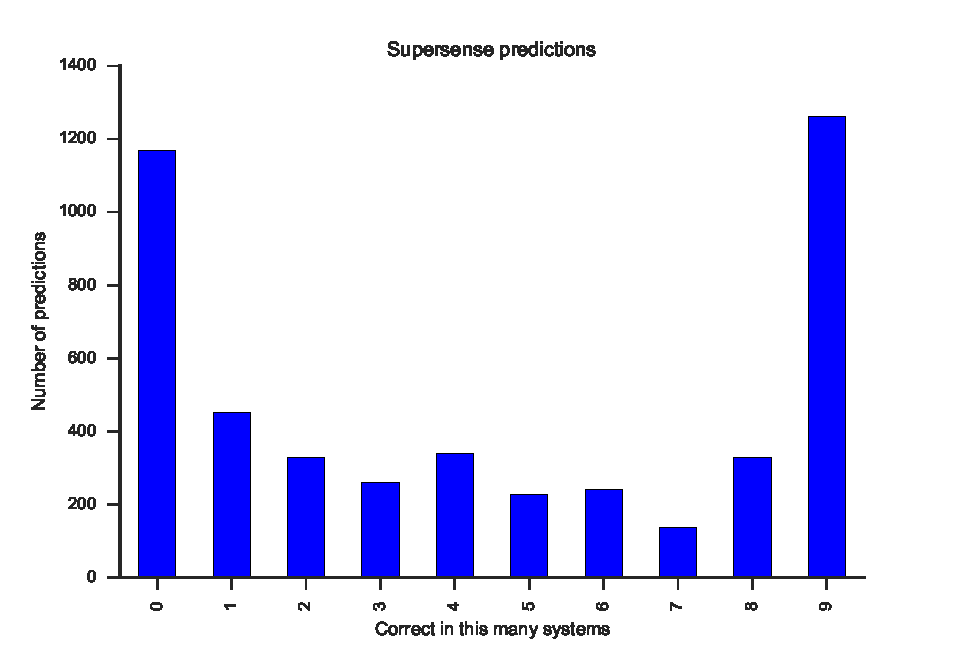
\includegraphics[width=8.5cm]{figs/supersense_predictions.pdf}
%	}
	\caption{Number of systems predicting the correct supersense (for tokens where there is a gold supersense). 
%\aj{Slight edit: the graph is not technically a histogram.}. \aj{I did try to produce a version with each bar split into domains. It turns out that there are practically no domain differences. Only thing I found was that Trustpilot supersenses have a slightly higher proportion of \emph{both} the easy and the hard cases. }
}
	\label{fig:supersense-predictions}
\end{figure}



\begin{figure}
%	\resizebox{ \columnwidth }{!}{
		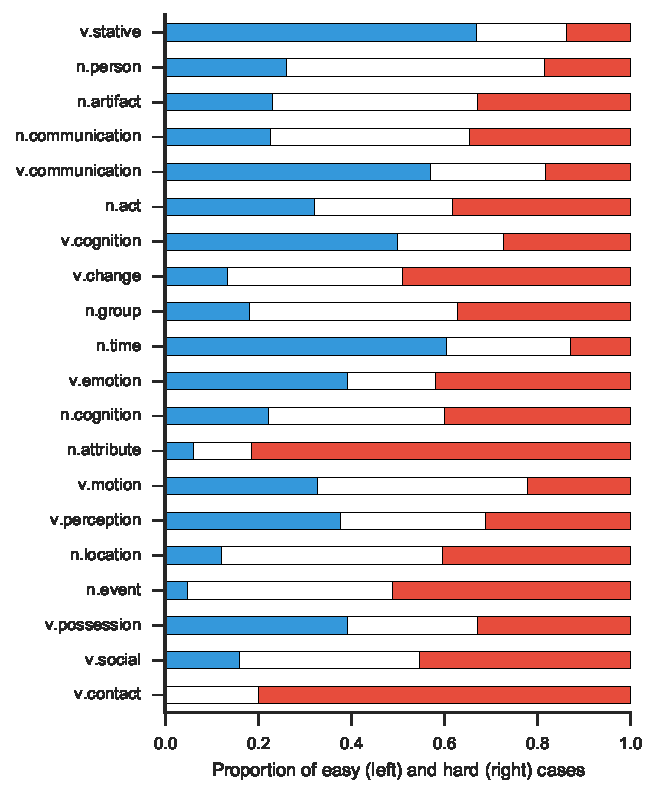
\includegraphics[width=8cm]{figs/proportion_of_easy_and_hard_supersenses.pdf}
%	}
	\caption{Easy and hard supersense decisions. Shown in blue in the left side of the plot is the proportion of instances of the given supersense type where at most one system gave the \emph{wrong} answer. On the right side in red is the corresponding figure where at most one system gave the \emph{right} answer. Supersenses are sorted by corpus frequency.}
	\label{fig:easy-and-hard-supersenses}
\end{figure}




\begin{figure}
	\resizebox{ \columnwidth }{!}{
		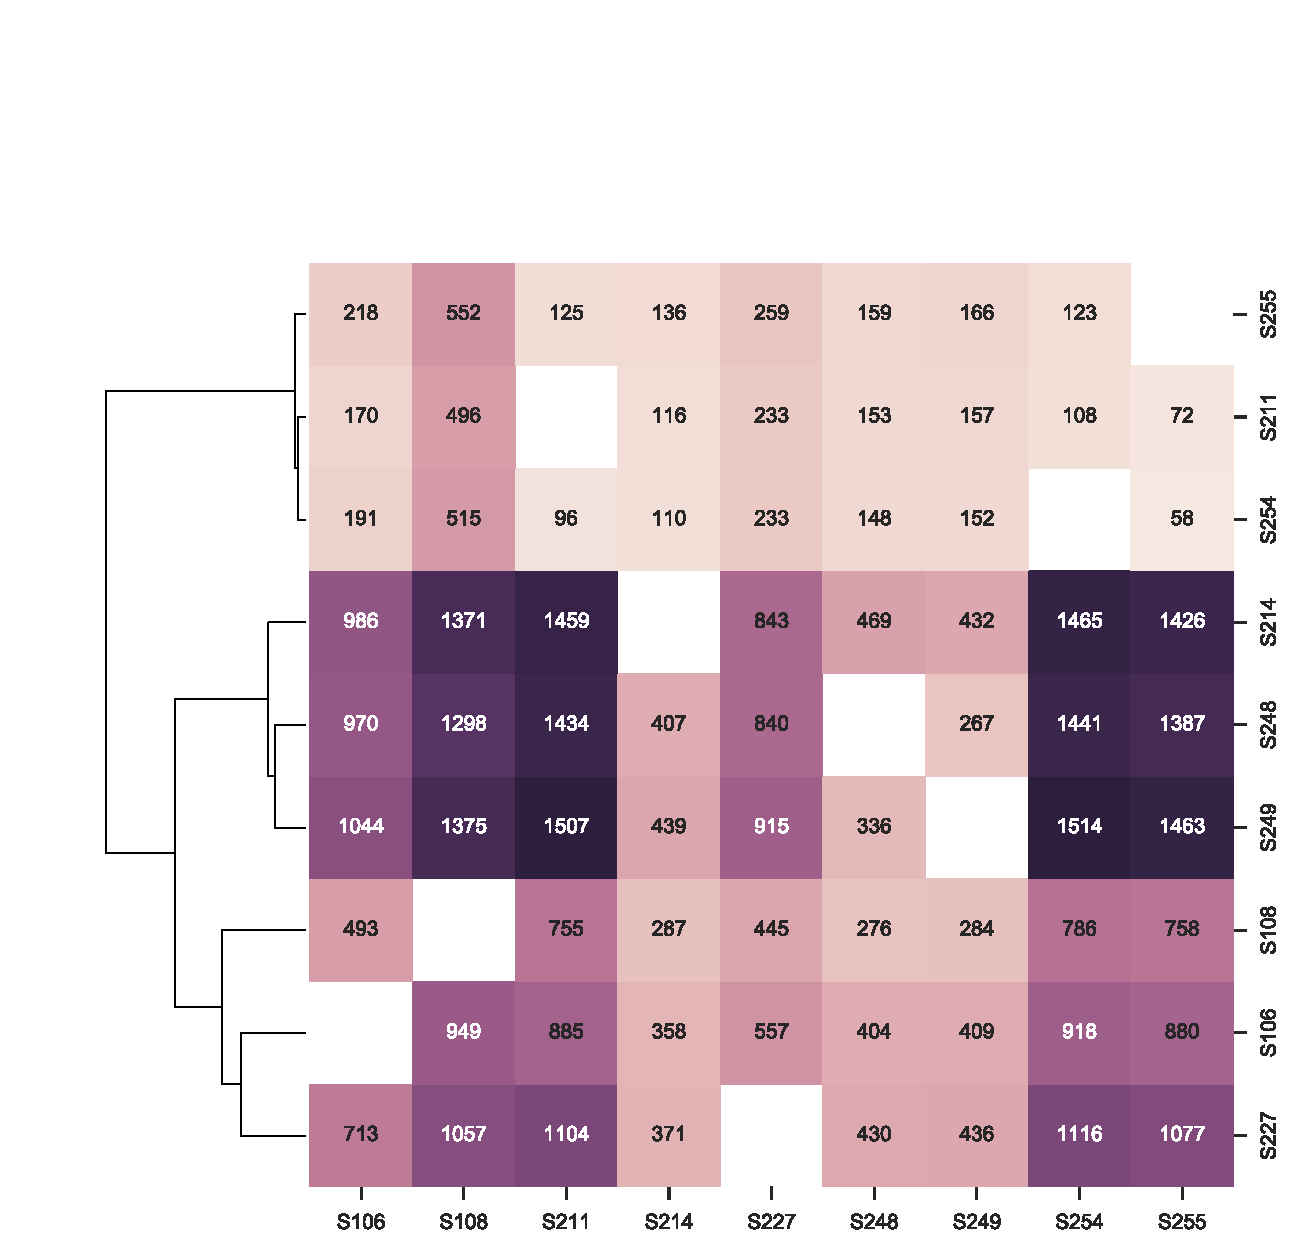
\includegraphics{figs/system_pairwise_clusters_cropped.pdf}
	}
	\caption{System clusters. Each cell compares the predictions of two systems $i$ and $j$ with respect to a gold standard. The value in the $i$,$j$-th cell is the number of predictions that $i$ got right but $j$ did not.}
	\label{fig:system-clusters}
\end{figure}













\section{Conclusion}
This task featured a broad-coverage lexical semantic analysis task that combines MWE identification and supersense tagging. 
The semantic tagset strikes a balance between the extremely difficult fine-grained distinctions in classical WSD, 
and the restrictiveness of the NER task. To guard against domain bias, we provided training data 
from two different genres, namely online reviews and tweets, as well as a test-only data set with TED talk transcripts. 

The best scoring system obtained .57 $F_1$ on a composite measure over the two subtasks of MWE and supersense tagging, 
averaged over the three test domains. This level of performance suggests that the task is not yet resolved. 
Furthermore, our error analysis suggested that the submitted systems to a large degree 
extracted the same knowledge from the training data. 
Substantial improvements of performance would thus seem to require novel approaches. 

\finalversion{
\section*{Acknowledgments}
\nss{Sam (annotator), funding}}

\begin{table}\small\centering
\begin{tabular}{lrrrr}
\toprule
{} &  Reviews &   \multicolumn{1}{c}{TED} &  Twitter &  \multicolumn{1}{c}{All} \\
Submission &          &       &          &             \\
\midrule
\multicolumn{5}{l}{\textbf{Multiword expressions}} \\

S106       &   0.4957 &  0.5676 &   0.5116 &      0.5148 \\
S108       &   0.2639 &  0.3344 &   0.3418 &      0.3098 \\
S211       &   0.0907 &  0.1828 &   0.1576 &      0.1346 \\
S214       &   0.5337 &  0.5714 &   0.5949 &      0.5666 \\
S227       &   0.3618 &  0.4176 &   0.3932 &      0.3849 \\
S248       &   0.5396 &  0.5235 &   0.5448 &      0.5393 \\
S249       &   0.5480 &  0.5348 &   0.6109 &      0.5724 \\
S254       &   0.0705 &  0.1630 &   0.0634 &      0.0820 \\
S255       &   0.0868 &  0.2011 &   0.1550 &      0.1348 \\[1.4ex]

\multicolumn{5}{l}{\textbf{Supersenses}} \\

S106       &   0.5093 &  0.4961 &   0.4920 &      0.4998 \\
S108       &   0.2582 &  0.2468 &   0.2463 &      0.2514 \\
S211       &   0.5200 &  0.5140 &   0.4995 &      0.5111 \\
S214       &   0.5766 &  0.6006 &   0.5599 &      0.5755 \\
S227       &   0.5136 &  0.5200 &   0.5170 &      0.5162 \\
S248       &   0.5719 &  0.5911 &   0.5682 &      0.5747 \\
S249       &   0.5700 &  0.5917 &   0.5746 &      0.5764 \\
S254       &   0.5268 &  0.5144 &   0.4966 &      0.5129 \\
S255       &   0.5198 &  0.5328 &   0.5111 &      0.5193 \\[1.4ex]

\multicolumn{5}{l}{\textbf{Combined score}} \\

S106       &   0.5071 &  0.5057 &   0.4954 &      0.5022 \\
S108       &   0.2586 &  0.2539 &   0.2587 &      0.2576 \\
S211       &   0.4619 &  0.4790 &   0.4442 &      0.4586 \\
S214       &   0.5698 &  0.5971 &   0.5663 &      0.5741 \\
S227       &   0.4925 &  0.5082 &   0.4974 &      0.4977 \\
S248       &   0.5666 &  0.5826 &   0.5638 &      0.5688 \\
S249       &   0.5661 &  0.5833 &   0.5818 &      0.5757 \\
S254       &   0.4657 &  0.4782 &   0.4299 &      0.4547 \\
S255       &   0.4615 &  0.4981 &   0.4544 &      0.4664 \\

\bottomrule
\end{tabular}

\caption{Per-domain evaluation results. Figures are $F_1$ percentages.\finalversion{\nss{show condition, bold statistical winners?}}}	
\label{tbl:per-domain-results}
\end{table}


\bibliographystyle{style/aclnat}
% you bib file should really go here
\setlength{\bibsep}{10pt}
{\fontsize{10}{12.25}\selectfont
\bibliography{dimsum}}



\end{document}
